%!TEX encoding = UTF-8 Unicode

Many waterfowl (Aves: Anatidae) species, like other groups of birds, have experienced population declines across North America, largely driven by habitat loss (Norton and Thomas~1994, Rosenberg et~al.~2019).  Active management to conserve North American waterfowl began during the late 19th century and has included international treaties, evolving hunting regulations, and public-private habitat manipulation (Williams et~al.~1999, Brasher et~al.~2019). As a result, population size of nearly 57\% of waterfowl species have increased, but more than 43\% remain in decline since 1970 (Rosenberg et~al.~2019). Annual fluctuation of population size for all waterfowl species suggests that continual monitoring and adjustments to management practices are still required  (Wilkins and Cooch~1999, Nichols et~al.~2007). 

	Successful waterfowl management requires detailed understanding of their reproductive biology but key aspects of the reproductive process are not fully understood. Accurate data at specific management locations are required for improvement (Nichols et~al.~1995, Hagy et~al.~2014). One location that has been continually managed for waterfowl reproduction is Duck Creek Conservation Area \textsc{(dcca)} in southeast Missouri. The area provides important foraging habitat during migration by controlling flooding to encourage plant growth. It also provides hollow tree cavities as well as nest boxes that mimic them to provide important spring nesting habitat for Hooded Merganser \textit{(Lophodytes cuculattus)} and Wood Duck \textit{(Aix sponsa).} To increase the understanding of waterfowl breeding at \textsc{dcca}, a study was conducted to compare nesting success by both species to habitat variables surrounding nest locations.  




\section*{Species background}

Hooded Merganser is a small diving duck (Figure~\ref{fig:hooded_merganser_photo}) native to North America. They are the only extant member of \textit{Lophodytes} and are most closely related to the typical mergansers of the genus \textit{Mergus}, such as the Common Merganser \textit{(M.~merganser)} and Red-breasted Merganser \textit{(M.~serrator)} in North America (Livezey 1995). Hooded Merganser is a small duck with a slender, serrated bill, and a pronounced crest on the head of both sexes. Females have a drab grey-brown body with a cinnamon crest. Males have a white chest, brown sides, a black back, and a black head with a prominent white patch on the crest. This crest can be raised or lowered in both sexes to alter the shape of the head and display a white color patch in males (Johnsgard 1961). 

\afterpage{%
\begin{figure}[p!]
	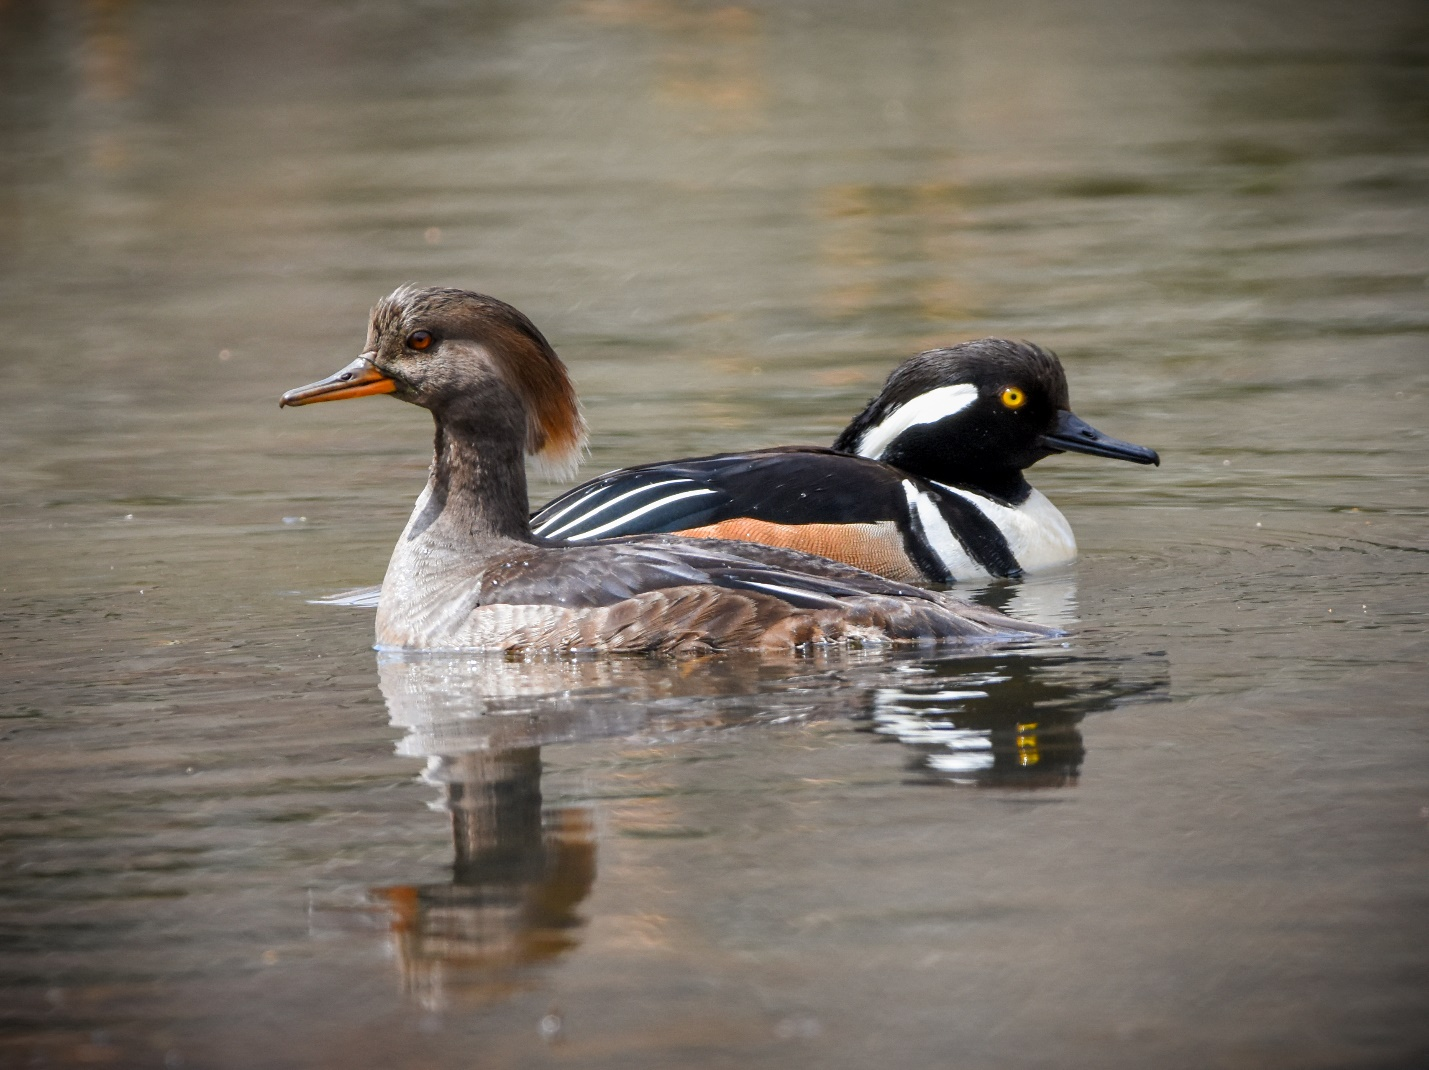
\includegraphics[width=\textwidth]{hooded_merganser_photo}
	\caption[Representative photo of Hooded Merganser]{Representative photo of Hooded Merganser hen (left) and drake (right). Photo by Jen Goellnitz, Flicker Creative Commons,  \ccbync{2.0}
	 \url{https://www.flickr.com/photos/goellnitz/33597600618/}.}
	\label{fig:hooded_merganser_photo}
\end{figure}
\clearpage}

 


Hooded Merganser dive below the water surface to sight feed for fishes, which dominate their diet, and invertebrates (Salyer and Lagler 1940, K. M. Dugger et~al.~1999). They favor water deep enough to support small fish or where they can swim below the surface, but their overall habitat includes ponds, rivers, large wetlands, and wooded swamps. The water bodies must have trees nearby because Hooded Merganser is a cavity nesters. Females lay eggs in hollow tree trunks above the ground or water. Courtship occurs before nesting and much earlier than other merganser species. The other, larger merganser species court during February, whereas Hooded Merganser begin courtship as early as November (Coupe and Cooke 1999). One male will pair with one female at least for the breeding season and egg laying will begin in March, earlier than many other cavity nesting waterfowl (Armbruster 1982, Rohwer and Anderson 1988, Soulliere and Rusch 1996, Rodway 2007). Hooded Merganser typically lays one clutch of 8–10 eggs per nesting season (Mallory et~al.~1998).  

Hooded Merganser has been negatively affected by habitat loss and alteration, largely due to clearcutting and draining fertile floodplain for industrial agriculture that results in the loss of permanent water and mature trees. As areas have been drained, Hooded Merganser has lost access to food sources. In areas not drained, timber harvesting and altered flood regimes have decreased the number of mature trees with suitable nesting cavities. Fewer cavities have reduced population growth compared to other waterfowl and seemingly increased the need for artificial nest boxes that mimic natural cavities to be included in management practices (Perry et~al.~2007).

One species competing with Hooded Merganser for nesting cavities is the Wood Duck.  Wood Duck is a small dabbling duck endemic to North America. Wood Duck is the only species of \textit{Aix} in North America. The only other species in the genus, the Mandarin Duck \textit{(Aix gtalericulata)}, is endemic to eastern Asia but is the sister species to Wood Duck (Liu et~al.~2014). Wood Duck have a short wide bill compared to that of the Hooded Merganser. Males are more variably colored than females with iridescent backs, brown chests, a red eye, and a small green crest on their heads (Figure~\ref{fig:wood_duck_photo}). Females are drabber in contrast being predominantly dull grey with a white eye stripe (Silvestro 2013). Wood Duck differs from Hooded Merganser in its food preference and foraging habit. Wood Duck is omnivorous and feed on small invertebrates during the breeding season with laying females eating up to 79\% animal matter (Landers et~al.~1977, Drobney and Fredrickson 1979). During the winter they are almost entirely herbivorous with up to 75\% of their food being acorns. Feeding is done by pecking on the surface or dabbling, with subsurface and bottoming feeding being rare. This makes them favor shallow water and edges in live-forest and emergent vegetation where surface level foods are abundant (Dugger and Fredrickson 1992).  

\afterpage{%
\begin{figure}[p!]
	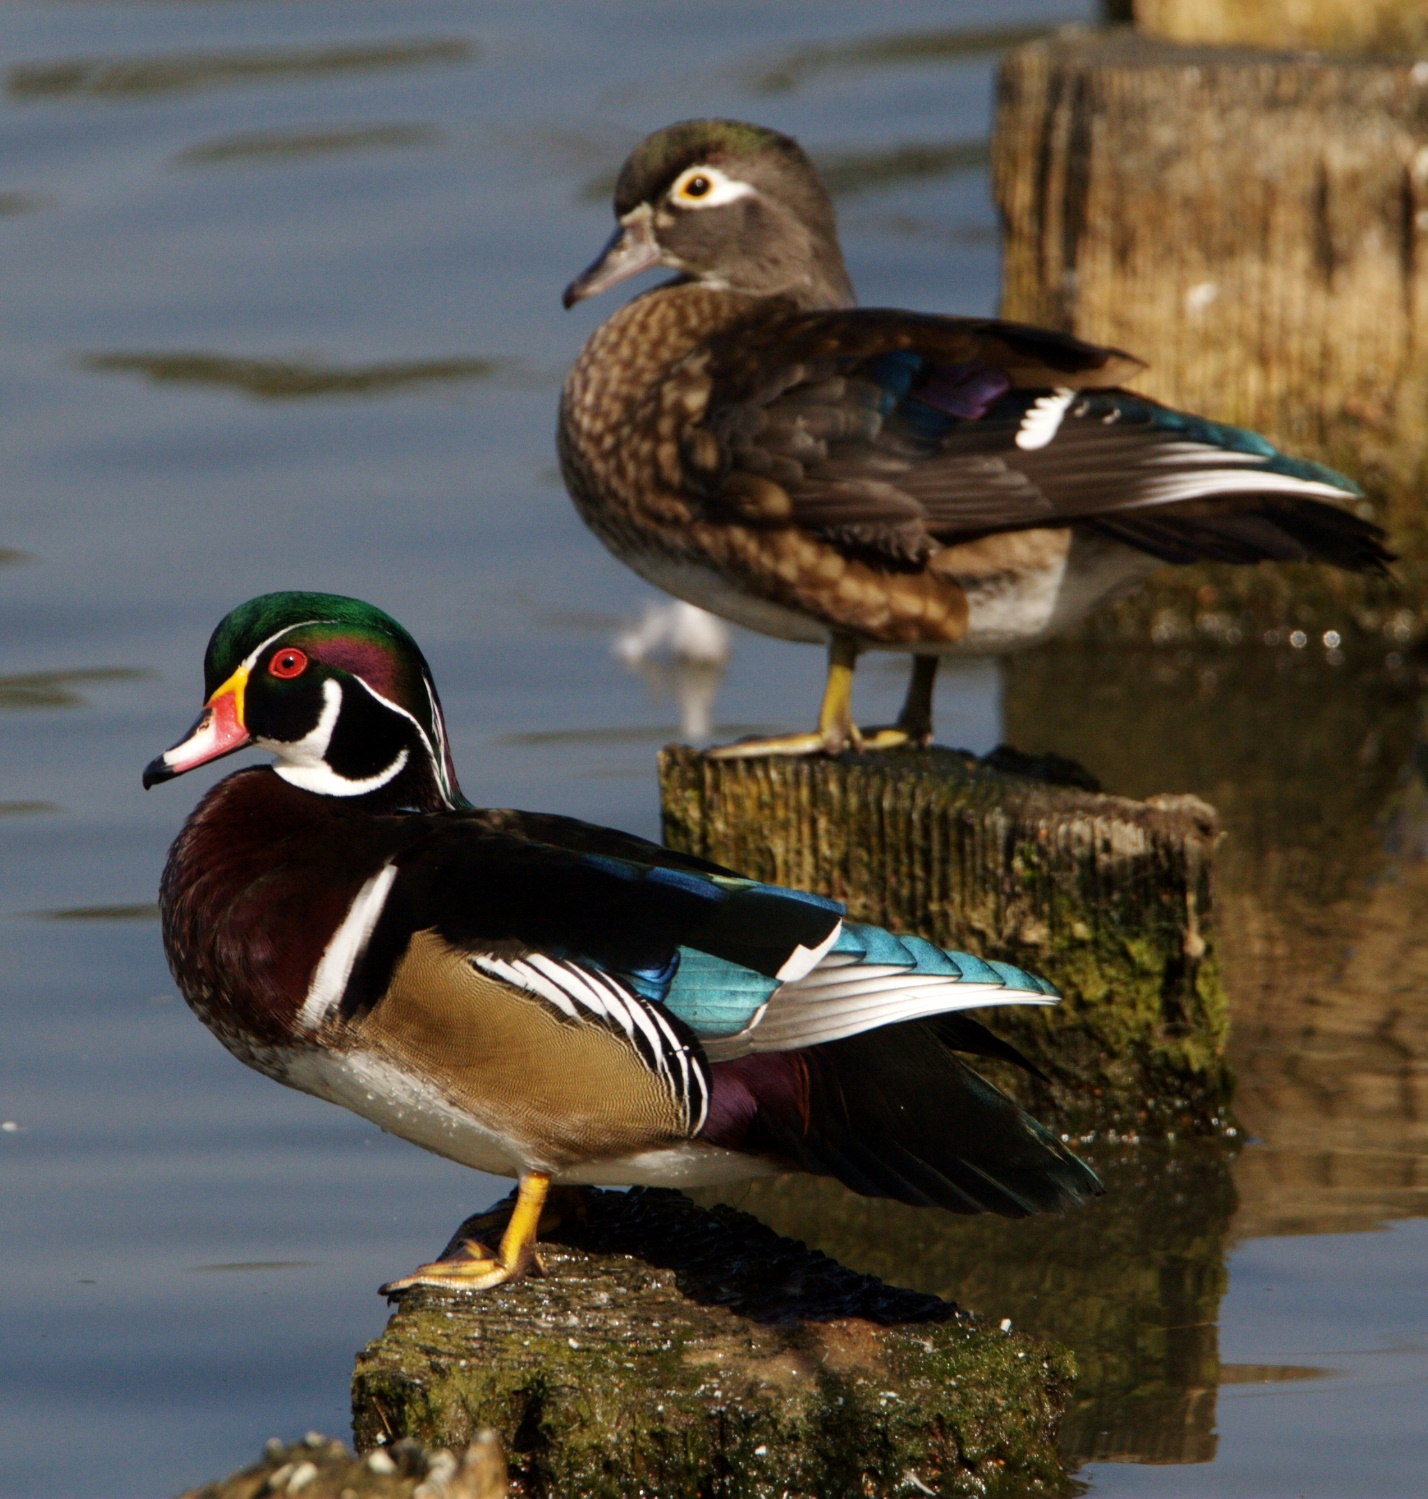
\includegraphics[width=\textwidth]{wood_duck_photo}
	\caption[Representative photo of Wood Duck]{Representative photo of Wood Duck drake (front) and hen (rear). Photo by Rick Leche – Photography, Flickr Creative Commons, \ccbyncnd{2.0} \url{https://www.flickr.com/photos/goellnitz/33597600618/}.}
	\label{fig:wood_duck_photo}
\end{figure}
\clearpage}
 

Like the Hooded Merganser, the Wood Duck constructs nests inside hollow tree cavities favoring similar habitat of swamps and sloughs with plentiful wooded cover, though they gravitate toward comparatively shallower areas (Bellrose et~al.~1964, Ryan et~al.~1998, Silvestro 2013). Wood Duck also courts early relative to other waterfowl beginning as early as September. Breeding pairs begin searching for nests in the early spring and have been observed to begin laying in early March (Armbruster 1982). Wood Duck lay an average of 12 eggs per clutch with numbers varying from 7 to 15 (Dugger and Fredrickson 1992, Semel and Sherman 1992). Wood Duck has also been shown to heavily utilize artificial nest boxes placed on the landscape to supplement natural cavities (Bellrose et~al.~1964, Scherpelz 1979, Ryan et~al.~1998).   

Nest boxes are man-made wooden boxes placed to mimic the natural tree cavities animals would use (Figure~\ref{fig:nest_box}). They do not have a standardized construction or system of placement, and often their location is chosen for ease of maintenance. Additionally, boxes are made in a variety of sizes with the entry hole regulating what species can access it. This results in those boxes used by Hooded Merganser and Wood Duck also being used by competing species such as Common Goldeneye \textit{(Bucephala clangula)}, owls, and potential predators such as racoons, snakes, and some woodpeckers (Heusmann and Stolarski 2017). It is unclear how the success of Hooded Merganser nests in boxes compare to those in natural cavities; research of other cavity-nesting bird species showed that different species had increased, similar, or decreased success in boxes compared to natural cavities (Purcell et~al.~1997).

\afterpage{%
\begin{figure}[p!]
	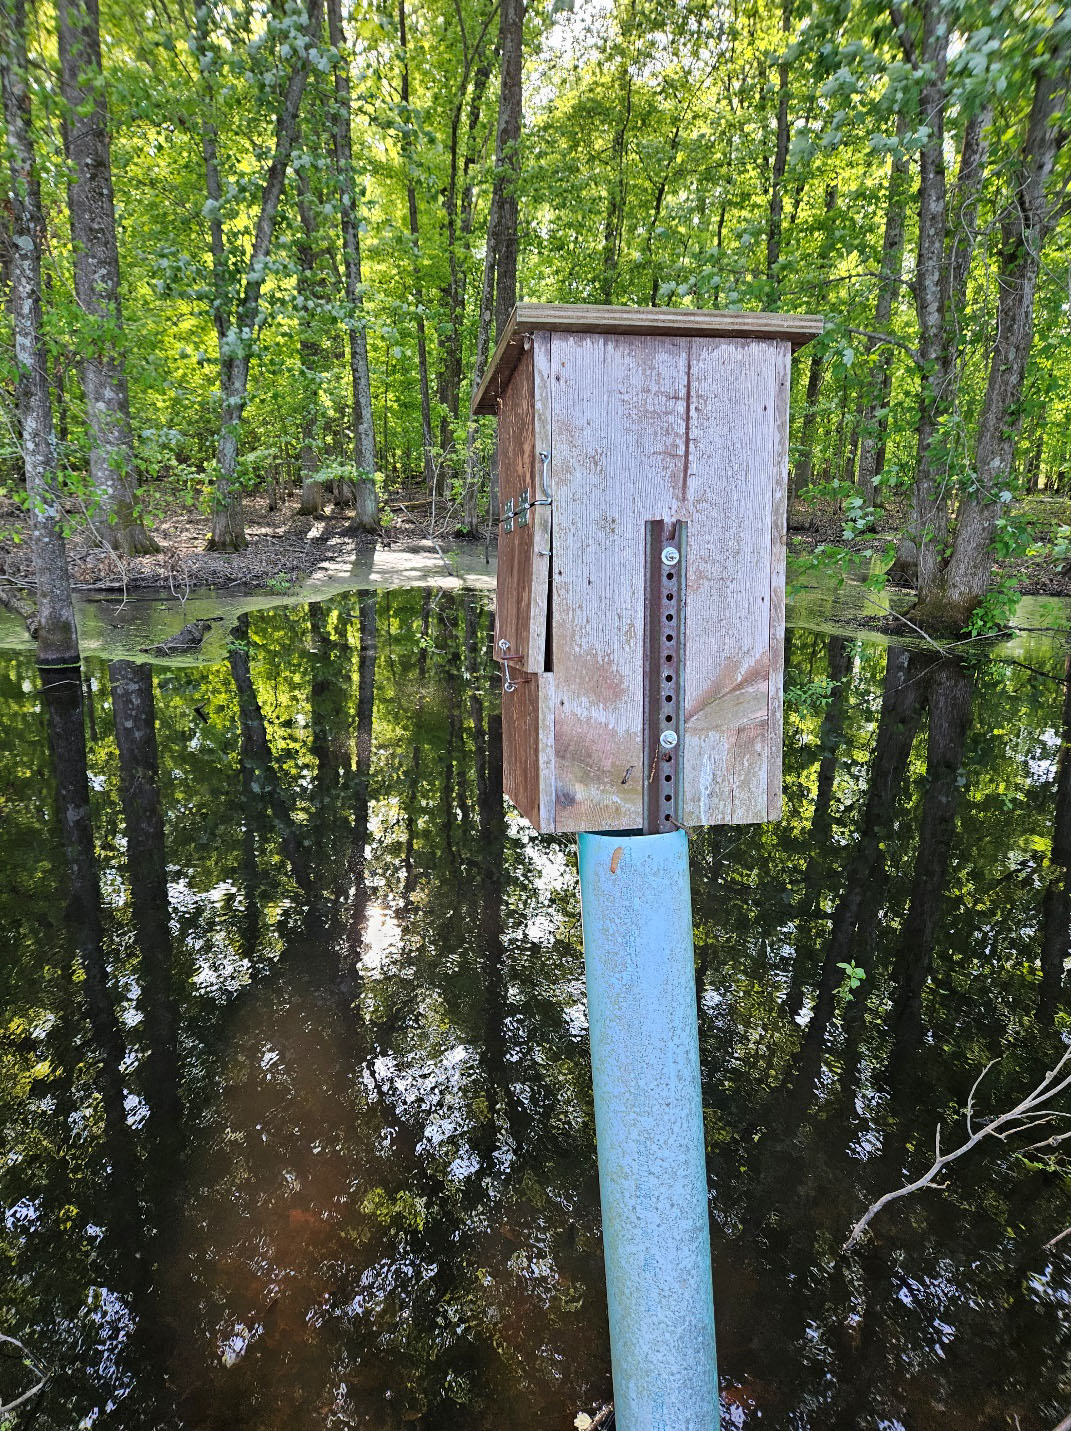
\includegraphics[height=0.85\textheight]{nest_box}
	\caption[Representative photograph of a nest box and surrounding habitat ]{Representative photograph of a nest box (S7) and surrounding habitat at Duck Creek Conservation Area, Puxico, Missouri. The door to access the nest is visible on the left side of the box. Photo by Frank J.~Irovic.}
	\label{fig:nest_box}
\end{figure}
\clearpage}
 


\section*{Prior research}

Nesting by the Hooded Merganser is little studied, usually in combination with other cavity-nesting species including Wood Duck (McNicol et~al.~1997, Mallory et~al.~2002). However, even these studies give valuable insight into merganser nesting. Previous studies have detailed general nesting behavior and success rates (Clawson et~al.~1979, Soulliere and Rusch 1996, Mallory et~al.~1998). Historical band-return data indicated that most mergansers returned to the same nesting locations each year, with 82\% of females nesting within one mile of their previous nest (Morse et~al.~1969). They initiated nesting in late February and mid-April with peak initiation occurring during March. They lay an average on one egg every 1.4–3 days, then line the nest with down and begin incubation. At the end of the approximately 28-day incubation period 80\% of Hooded Merganser nests studied successfully hatched young (Morse et~al.~1969, SénéChal et~al.~2008).  

One study (Ludt~2003) of 40 nest boxes on the same management area found nest box use increased from 21\% in 1994 to 33\% in 1998 but hatching success decreased from 90\% to 79\%. This may have been due to increased brood parasitism from 13\% to 75\% along with the increased nest box use (Ludt~2003). Nest success may also be negatively affected by dump nesting, a common form of brood parasitism that entails a female laying their eggs in another female’s nest. It is a common occurrence in birds with approximately 75 species making no nest and relying solely on dumping for reproduction (Hamilton and Orians 1965). Eggs dumped into Hooded Merganser nests may be from conspecifics or other species including Wood Duck and Common Goldeneye. Hens will displace dumped eggs to the periphery of the nest, potentially reducing their incubation efficiency (B. D. Dugger et~al.~1999).  In one study of Wood Duck, non-parasitized nests showed 78\% of eggs present hatched compared to only 63\% of eggs in parasitized nests (Clawson et~al.~1979). However, another study noted that despite similar negative effects on nest survival rates, interspecific brood parasitism minimally impacted Wood Duck breeding productivity (Bakner et~al.~2024). No comparable studies of the effects of dump nesting on Hooded Merganser have apparently been performed.

Additional research focused on the nest boxes themselves and their surrounding habitat. The use of nest boxes increased nest density compared to before box use. Nest boxes also increased the number of eggs per clutch, with the largest clutch increasing from 16 to 24 eggs from 1981–1985 (Zicus 1990).  Nest boxes might increase vulnerability to predation, which has been shown to impact up to 50\% of nests (Christman and Dhondt 1997, Pöysä et~al.~1997). Racoons successfully destroyed 43\% of Wood Duck nest boxes without predator guards but were unable to invade a single box (0\%) with predator guards (Lacki et~al.~1987). In contrast, the Black Rat Snake can circumvent predator guards to consume eggs and sometimes kill incubating Hooded Merganser hens (Fendley 1980).  


Few studies have addressed the habitat parameters that influence Hooded Merganser and Wood Duck choice among available nest boxes.  Hooded Merganser targets food sources by diving so they likely would favor deeper water, as it would allow for more efficient foraging while laying and incubating eggs. In contrast, the Wood Duck habit of foraging at or near the surface may make shallower water more advantageous for them. Due to foraging differences, I predicted that Hooded Merganser would use artificial nest boxes located near deep water but Wood Duck would favor shallower water. To test this prediction artificial nest boxes at Duck Creek Conservation Area in southeast Missouri were surveyed during the spring and summer of 2024.  Water width and tree coverage within 100 m\textsuperscript{2} were also measured because they might also influence nest box choice. 

